\PassOptionsToPackage{unicode=true}{hyperref} % options for packages loaded elsewhere
\PassOptionsToPackage{hyphens}{url}
%
\documentclass[]{article}
\usepackage{lmodern}
\usepackage{amssymb,amsmath}
\usepackage{ifxetex,ifluatex}
\usepackage{fixltx2e} % provides \textsubscript
\ifnum 0\ifxetex 1\fi\ifluatex 1\fi=0 % if pdftex
  \usepackage[T1]{fontenc}
  \usepackage[utf8]{inputenc}
  \usepackage{textcomp} % provides euro and other symbols
\else % if luatex or xelatex
  \usepackage{unicode-math}
  \defaultfontfeatures{Ligatures=TeX,Scale=MatchLowercase}
\fi
% use upquote if available, for straight quotes in verbatim environments
\IfFileExists{upquote.sty}{\usepackage{upquote}}{}
% use microtype if available
\IfFileExists{microtype.sty}{%
\usepackage[]{microtype}
\UseMicrotypeSet[protrusion]{basicmath} % disable protrusion for tt fonts
}{}
\IfFileExists{parskip.sty}{%
\usepackage{parskip}
}{% else
\setlength{\parindent}{0pt}
\setlength{\parskip}{6pt plus 2pt minus 1pt}
}
\usepackage{hyperref}
\hypersetup{
            pdfborder={0 0 0},
            breaklinks=true}
\urlstyle{same}  % don't use monospace font for urls
\usepackage{graphicx,grffile}
\makeatletter
\def\maxwidth{\ifdim\Gin@nat@width>\linewidth\linewidth\else\Gin@nat@width\fi}
\def\maxheight{\ifdim\Gin@nat@height>\textheight\textheight\else\Gin@nat@height\fi}
\makeatother
% Scale images if necessary, so that they will not overflow the page
% margins by default, and it is still possible to overwrite the defaults
% using explicit options in \includegraphics[width, height, ...]{}
\setkeys{Gin}{width=\maxwidth,height=\maxheight,keepaspectratio}
\setlength{\emergencystretch}{3em}  % prevent overfull lines
\providecommand{\tightlist}{%
  \setlength{\itemsep}{0pt}\setlength{\parskip}{0pt}}
\setcounter{secnumdepth}{0}
% Redefines (sub)paragraphs to behave more like sections
\ifx\paragraph\undefined\else
\let\oldparagraph\paragraph
\renewcommand{\paragraph}[1]{\oldparagraph{#1}\mbox{}}
\fi
\ifx\subparagraph\undefined\else
\let\oldsubparagraph\subparagraph
\renewcommand{\subparagraph}[1]{\oldsubparagraph{#1}\mbox{}}
\fi

% set default figure placement to htbp
\makeatletter
\def\fps@figure{htbp}
\makeatother


\date{}

\begin{document}

\#\#\# Sistemi Operativi \#\#\# Unità 1: Introduzione Introduzione ai
Sistemi Operativi =====================
\href{https://trevisan.inginf.units.it/}{Martino Trevisan}
\href{https://www.units.it}{Università di Trieste}
\href{https://dia.units.it/}{Dipartimento di Ingegneria e Architettura}

\hypertarget{componenti-di-un-sistema-di-elaborazione}{%
\subsection{Componenti di un sistema di
elaborazione}\label{componenti-di-un-sistema-di-elaborazione}}

Un sistema di elaborazione si può suddividere in quattro componenti: -
Hardware - Fornisce le risorse fisiche: CPU, memoria, disco - Sistema
Operativo - Gestisce l'accesso all'hardware da parte dei programmi -
Programmi Applicativi - Eseguono i compiti desiderati dagli utenti o dal
sistema - Utenti - Lanciano e usano programmi

\hypertarget{architettura-di-un-sistema-di-elaborazione}{%
\subsection{Architettura di un sistema di
elaborazione}\label{architettura-di-un-sistema-di-elaborazione}}

\begin{itemize}
\tightlist
\item
  La CPU esegue le istruzioni che preleva dalla memoria.
\item
  Moduli fondamentali:

  \begin{itemize}
  \tightlist
  \item
    Arithmetic Logic Unit
  \item
    Control Unit
  \item
    Registri
  \end{itemize}
\item
  Tre fasi per eseguire ogni istruzione
\end{itemize}

\begin{figure}
\centering
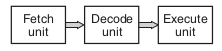
\includegraphics{images/cpu.png}
\caption{width:300px center}
\end{figure}

\hypertarget{architettura-di-un-sistema-di-elaborazione-1}{%
\subsection{Architettura di un sistema di
elaborazione}\label{architettura-di-un-sistema-di-elaborazione-1}}

\begin{itemize}
\tightlist
\item
  Un sistema di elaborazione interagisce con l'esterno tramite
  dispositivi di Input/Output

  \begin{itemize}
  \tightlist
  \item
    Schermo
  \item
    Tastiera
  \item
    Mouse
  \item
    Rete
  \item
    Sensori
  \end{itemize}
\item
  Comunicano con la CPU tramite il bus
\end{itemize}

\begin{figure}
\centering
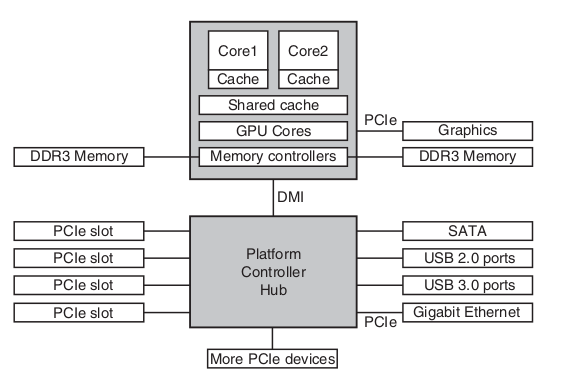
\includegraphics{images/io.png}
\caption{width:350px bg auto right:35\%}
\end{figure}

\hypertarget{definizione-di-sistema-operativo}{%
\subsection{Definizione di sistema
operativo}\label{definizione-di-sistema-operativo}}

\begin{itemize}
\tightlist
\item
  In un certo senso, i sistemi operativi rendono gradevole ciò che ha
  un'interfaccia sgradevole
\end{itemize}

\begin{figure}
\centering
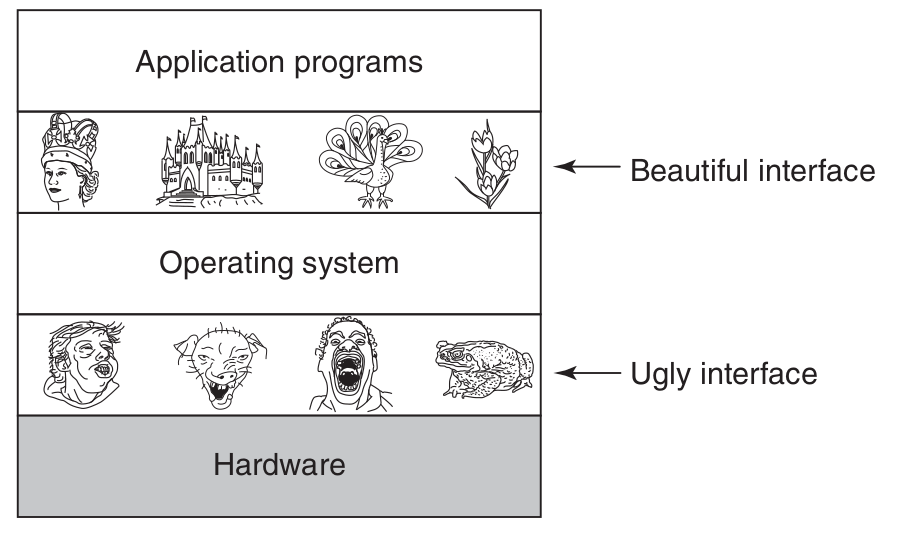
\includegraphics{images/so-beauty.png}
\caption{width:500px center}
\end{figure}

\hypertarget{componenti-di-un-sistema-operativo}{%
\subsection{Componenti di un sistema
operativo}\label{componenti-di-un-sistema-operativo}}

\begin{itemize}
\tightlist
\item
  Un sistema di elaborazione è composto di diversi moduli

  \begin{itemize}
  \tightlist
  \item
    Che offrono servizi a utente
  \item
    Ma interagiscono anche tra loro
  \end{itemize}
\end{itemize}

\begin{figure}
\centering
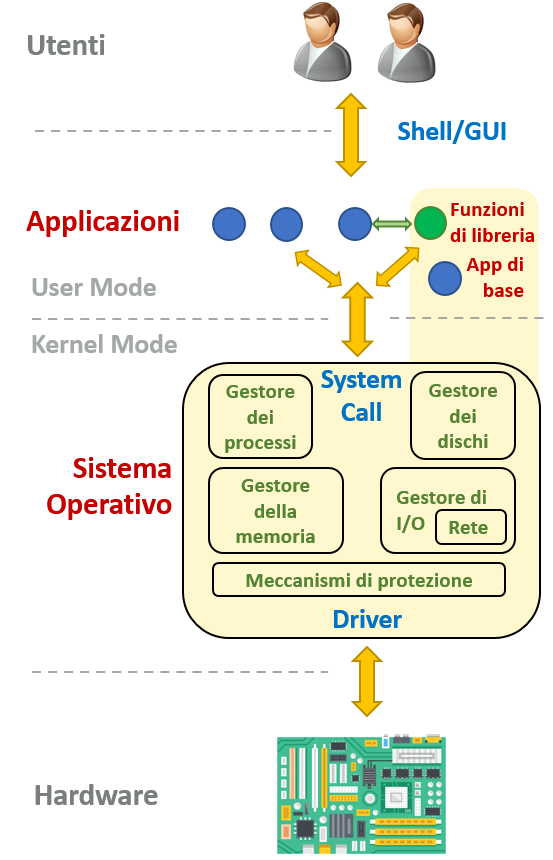
\includegraphics{images/so-scheme.png}
\caption{width:350px bg auto right:40\%}
\end{figure}

\hypertarget{componenti-di-un-sistema-operativo-1}{%
\subsection{Componenti di un sistema
operativo}\label{componenti-di-un-sistema-operativo-1}}

\begin{itemize}
\tightlist
\item
  \textbf{Gestore dei dispositivi di I/O}:

  \begin{itemize}
  \tightlist
  \item
    I dispositivi di I/O non sono gestiti direttamente dalle
    applicazioni

    \begin{itemize}
    \tightlist
    \item
      Sarebbe complicato e creerebbe problemi di funzionamento
    \end{itemize}
  \item
    I SO utilizza i driver per pilotare i dispositivi
  \item
    La connessione di rete rappresenta un caso particolare di I/O.

    \begin{itemize}
    \tightlist
    \item
      Ha un trattamento speciale nei moderni SO
    \end{itemize}
  \end{itemize}
\item
  \textbf{Gestore dei meccanismi di protezione}:

  \begin{itemize}
  \tightlist
  \item
    Nei SO ci sono tanti utenti con diversi permessi di accedere alle
    risorse

    \begin{itemize}
    \tightlist
    \item
      Per accedere a file, dispositivi, configurazione, ecc\ldots{}
    \end{itemize}
  \item
    I SO implementa le policy di accesso
  \end{itemize}
\end{itemize}

\hypertarget{definizioni-relative-ai-sistemi-operativi}{%
\subsection{Definizioni relative ai sistemi
operativi}\label{definizioni-relative-ai-sistemi-operativi}}

\begin{itemize}
\tightlist
\item
  \textbf{Kernel}:

  \begin{itemize}
  \tightlist
  \item
    Cuore del SO
  \item
    Include tutti i moduli visti in precedenza

    \begin{itemize}
    \tightlist
    \item
      Gestisce le operazioni fondamentali e a più basso livello
    \end{itemize}
  \item
    Modulo software sempre in esecuzione

    \begin{itemize}
    \tightlist
    \item
      Con privilegi speciali
    \item
      Tutte le altre applicazioni (di utente o di sistema) hanno
      privilegi minori

      \begin{itemize}
      \tightlist
      \item
        Si appoggiano al kernel
      \end{itemize}
    \end{itemize}
  \item
    Diverse tipologie di kernel

    \begin{itemize}
    \tightlist
    \item
      Monolitici: il kernel è un unico programma che esegue tutto il
      codice necessario

      \begin{itemize}
      \tightlist
      \item
        I più comuni
      \end{itemize}
    \item
      Micro-Kernel: cercano di delegare alle applicazioni più
      funzionalità possibile
    \item
      A livelli stratificati: il kernel (e i programmi) sono organizzati
      in una gerarchia di processi a privilegi crescenti.
    \end{itemize}
  \end{itemize}
\end{itemize}

\hypertarget{definizioni-relative-ai-sistemi-operativi-1}{%
\subsection{Definizioni relative ai sistemi
operativi}\label{definizioni-relative-ai-sistemi-operativi-1}}

\begin{itemize}
\tightlist
\item
  \textbf{System call}:

  \begin{itemize}
  \tightlist
  \item
    Sono delle funzioni messe a disposizione dal SO alle applicazioni
  \item
    Offrono i servizi del SO per creare processi, accedere ai dischi,
    ecc\ldots{}

    \begin{itemize}
    \tightlist
    \item
      Il kernel ``serve'' le richieste di System Call dei programmi
    \end{itemize}
  \item
    Da non confondere con le Funzioni di Libreria

    \begin{itemize}
    \tightlist
    \item
      Che sono moduli software che svolgono compiti comuni a più
      applicazioni
    \item
      Sono software comuni con stessi privilegi di applicazione
    \item
      Possono (ma non sempre) chiamare delle System Call
    \end{itemize}
  \end{itemize}
\end{itemize}

\hypertarget{definizioni-relative-ai-sistemi-operativi-2}{%
\subsection{Definizioni relative ai sistemi
operativi}\label{definizioni-relative-ai-sistemi-operativi-2}}

\begin{itemize}
\tightlist
\item
  \textbf{System call}:

  \begin{itemize}
  \tightlist
  \item
    Esempi di System Call comuni:

    \begin{itemize}
    \tightlist
    \item
      Gestione dei process: \texttt{fork} \texttt{exec} \texttt{wait}
      \texttt{kill}
    \item
      Gestione dei file: \texttt{open} \texttt{close} \texttt{read}
      \texttt{write}
    \end{itemize}
  \item
    Nota: i SO operativi offrono anche molte funzioni di libreria

    \begin{itemize}
    \tightlist
    \item
      Alcune funzioni di libreria non necessitano di System Call
    \item
      Calcolare la radice quadrata: \texttt{double\ sqrt(double\ arg)}.
      Non necessita di una System Call
    \item
      Scrivere su schermo:
      \texttt{int\ printf(char\ *format,\ arg\ list\ ...)}. Formatta la
      stringa da scrivere e poi chiama la System Call \texttt{write}
    \end{itemize}
  \end{itemize}
\end{itemize}

\hypertarget{definizioni-relative-ai-sistemi-operativi-3}{%
\subsection{Definizioni relative ai sistemi
operativi}\label{definizioni-relative-ai-sistemi-operativi-3}}

\begin{itemize}
\tightlist
\item
  \textbf{File System}:

  \begin{itemize}
  \tightlist
  \item
    Struttura che include un insieme di file e cartelle
  \item
    Organizzato secondo un albero
  \end{itemize}
\end{itemize}

\begin{figure}
\centering
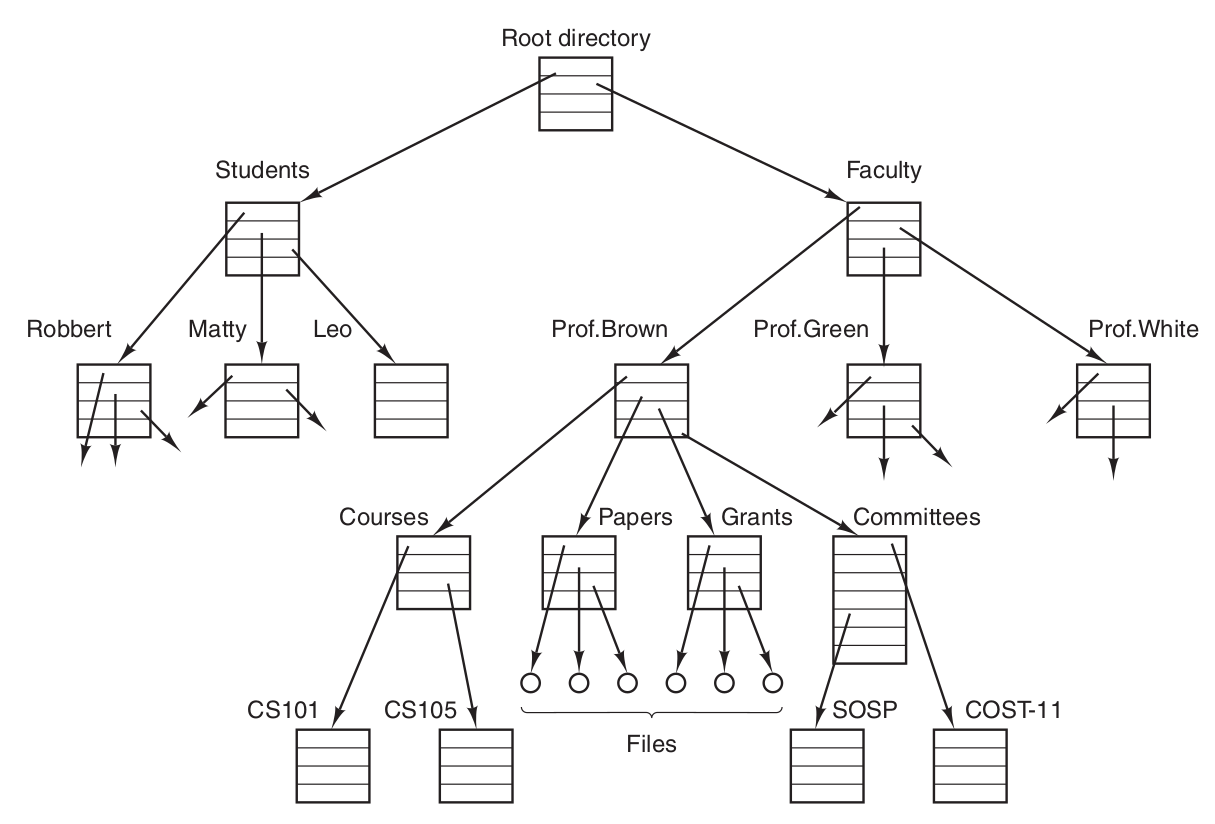
\includegraphics{images/tree.png}
\caption{width:600px center}
\end{figure}

\hypertarget{definizioni-relative-ai-sistemi-operativi-4}{%
\subsection{Definizioni relative ai sistemi
operativi}\label{definizioni-relative-ai-sistemi-operativi-4}}

\begin{itemize}
\tightlist
\item
  \textbf{Bootloader}:

  \begin{itemize}
  \tightlist
  \item
    Il codice che carica in memoria il kernel al momento dell'accensione
    del sistema
  \item
    Contenuto in ROM/EEPROM
  \end{itemize}
\item
  \textbf{Login}:

  \begin{itemize}
  \tightlist
  \item
    Autenticazione di un utente nel sistema, solitamente tramite
    username e password
  \end{itemize}
\item
  \textbf{Shell}:

  \begin{itemize}
  \tightlist
  \item
    Programma che legge comandi da tastiera, li esegue e ne stampa
    l'output
  \item
    Metodo di accesso tradizionale
  \item
    Non fa parte del kernel

    \begin{itemize}
    \tightlist
    \item
      Quando un sistema viene avviato, il kernel avvia sempre una shell
      o l'interfaccia grafica
    \end{itemize}
  \end{itemize}
\end{itemize}

\begin{center}\rule{0.5\linewidth}{0.5pt}\end{center}

\hypertarget{domande}{%
\subsection{Domande}\label{domande}}

Cosa é un processo? \texttt{•\ Un\ programma} \texttt{•\ Un\ algoritmo}
\texttt{•\ Un\ programma\ in\ esecuzione}

Le System Call sono usate da:
\texttt{•\ SO\ per\ interagire\ con\ l\textquotesingle{}hardWare}
\texttt{•\ Dai\ processi\ per\ interagire\ col\ SO}

Le Funzioni di Libreria vengono eseguite: \texttt{•\ In\ User\ Mode}
\texttt{•\ In\ Kernel\ Mode}

Il File System é organizzato come:
\texttt{•\ Un\ Grafo\ contentente\ cicli}
\texttt{•\ Un\ Grafo\ NON\ contentente\ cicli}

\end{document}
